\chapter{4-quadrant chopper used in railway traction}
% Sources: https://www.techniques-ingenieur.fr/base-documentaire/ingenierie-des-transports-th14/materiel-roulant-ferroviaire-42630210/tramways-c4442/performances-en-traction-et-en-freinage-c4442niv10003.html

\textit{The reversible structure of this type of chopper allows for its use in controlling direct current machines in traction, where reversibility is most interesting to exploit. It is used for all power ranges, with the example given here being that of a tramway.}

The tramway is modeled by a "car" powered by a DC machine, itself controlled by a reversible chopper powered by a perfect reversible DC source (catenary type). The simplified diagram of the device is shown in the following figure and corresponds to the described quantities.

\begin{figure}[H]
\centering
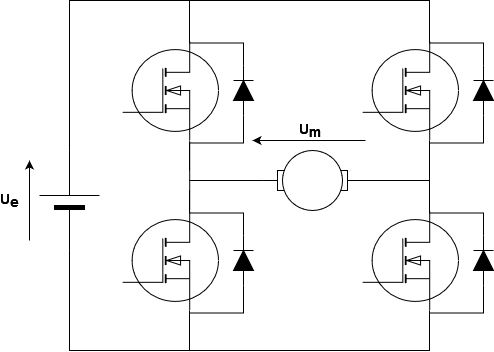
\includegraphics[width=0.55\linewidth]{TD_H4Q/fig/H4Q.png}
\caption{4 Quadrant chopper}
\end{figure}

The chopper is powered by a constant voltage source with a value of $U_E = 1500 V$. It consists of two independent bridge arms controlled at a fixed frequency of $F_d = 2 kHz$. The duty cycles are denoted as follows: $\alpha_1$ for $T_{11}$ and $\alpha_2$ for $T_{21}$, with the control of each arm being complementary. We assume perfect components, diodes, and transistors. Between the two bridge arms, the following control relationship is maintained: $\alpha_1 + \alpha_2 = 1$.

The direct current motor is conventionally modeled by its electromotive force (EMF) $E$, its armature resistance $R$, and its armature inductance $L$; its excitation is kept constant by another device not studied here. The torque constant (equal to the EMF constant) is denoted as $k_\varphi$, and the numerical values are as follows:

$R = 0.2 \Omega$; $L = 25 mH$; $k_\varphi = 7.64 Nm/A$; nominal speed $N_n = 1500 rpm$.

The tramway car constitutes the mechanical load and presents, with respect to the motor shaft, a moment of inertia $J = 200 kg.m^2$. Depending on the trajectory, it also "returns" to this motor shaft a resisting torque denoted as $C_v$.

\begin{enumerate}
\item \textbf{Total complementary control}

\begin{enumerate}
\item Quickly represent the shape of the motor voltage $u_m(t)$ for any duty cycle $\alpha_1$, first less than $0.5$ and then greater than $0.5$.
\item Calculate the average value of this voltage, denoted as $U_m$, as a function of $\alpha_1$.
\end{enumerate}

\item \textbf{Functional description}

In this part, we neglect the current ripple in the motor. In addition, a very fast current control compared to the mechanical time constants allows us to impose the desired value on the motor armature current, denoted as $I_M$, which is constant.

\begin{enumerate}
\item Express the average values (at the switching frequency $F_d$) of the voltage across the motor armature, denoted as $U_M$, and the current drawn by the chopper from the source, denoted as $I_E$, as functions of $\alpha_1$, $U_E$, and $I_M$.
\item The tramway stops on an \textbf{uphill} slope. The weight of the car then exerts a torque on the motor shaft with a value of $C_v = 382 Nm$. What is the duty cycle $\alpha_{10}$ required to keep the tramway at a standstill? What is the current $I_{E0}$ drawn from the power supply (still in average value)?
\item The tramway starts on a level track (neglecting the resisting torque) with a constant acceleration of $5 rad/s^2$ until it reaches the nominal motor speed.

\begin{enumerate}
\item What is the current $I_m$ in the motor?
\item Plot the variation of the duty cycle $\alpha_{1}$ during this acceleration phase.
\item Plot the variation of the current $I_E$ drawn from the power supply during this acceleration phase.
\item Calculate the acceleration time $\Delta t_a$.
\end{enumerate}

\item The tramway travels on a \textbf{downhill} trajectory at a constant speed, with the motor running at its nominal speed. The weight exerts a torque $C_v = 382 Nm$. What is the current $I_{Ed}$ drawn from the power supply? What is the value of the duty cycle $\alpha_{1d}$ that allows for this constant speed operation?
\item Emergency braking downhill: during the previous operation (1.3), the driver requests emergency braking characterized by controlling the armature current to the maximum value tolerable by the chopper and the machine, $I_{max} = 250 A$. We assume that this current is imposed quasi-instantaneously and remains present during the deceleration phase, with the torque related to the weight of the car remaining unchanged at $382 Nm$.

\begin{enumerate}
\item Calculate and represent the time evolution of the motor speed $\Omega(t)$, which represents the tramway speed.
\item Calculate the deceleration time until stop, denoted as $\Delta t_a$.
\item Determine the evolution of the duty cycle $\alpha_1(t)$ during this phase, specifying its value at the beginning of braking and just before the vehicle comes to a stop.
\item Calculate the total energy $E_C$ returned to the source during this braking operation.
\end{enumerate}

\item Represent the operating quadrants of the chopper used during the different phases of the tramway operation.
\end{enumerate}

% \newpage
% \item \textbf{Shifted complementary control of the chopper}

% Here, we propose to change the control of the switches. It is performed according to the diagram shown in the following figure. For each "bridge arm", the control is still complementary with a frequency of $F_d$ (assuming instantaneous switching). To achieve the modulation of the duty cycle, a comparison is made between a modulator ($M_1$ or $M_2$) and the voltage representing the duty cycle $\alpha$, denoted as $v_{alpha}$. We assume that the output of these comparators is a binary signal used to control the switches.

% \begin{figure}[H]
% \centering
% 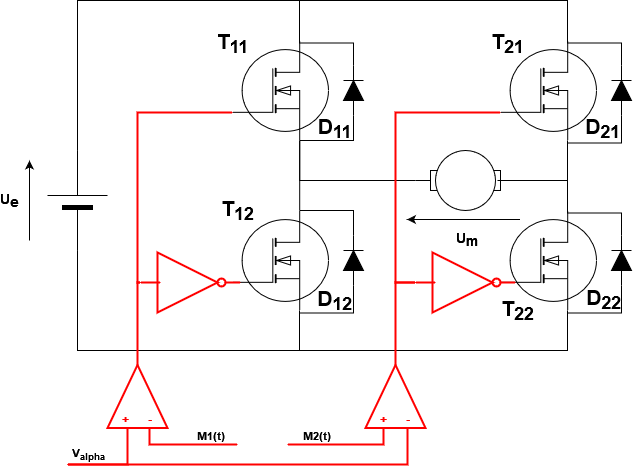
\includegraphics[width=0.6\linewidth]{TD_H4Q/fig/H4Q_decale.png}
% \caption{Shifted control of a 4 quadrant chopper}
% \end{figure}

% The two modulators are shown in the following figure: they are triangular signals in phase opposition with an amplitude of $1 V$. The signal $v_{alpha}$ itself has a maximum amplitude of $1 V$, with its actual amplitude being proportional to the duty cycle $\alpha$.

% \begin{enumerate}
% \item For $\alpha = 0.8$, represent the switching functions $f_1(t)$ and $f_2(t)$ as well as the motor voltage $u_m(t)$.
% \item What is the frequency of the signal $u_m$? What is its "duty cycle", denoted as $\beta$?
% \item For $\alpha = 0.2$, represent the switching functions $f_1(t)$ and $f_2(t)$ as well as the motor voltage $u_m(t)$.
% \item When $\alpha$ is between 0.5 and 1, neglecting the resistance $R$, determine the ripple $\Delta I_M$ in the motor current. What is its maximum value $\Delta I_{M max}$?
% \item What is the advantage of this control compared to total complementary control?
% \end{enumerate}


% \newpage
% \begin{figure}[H]
% \centering
% 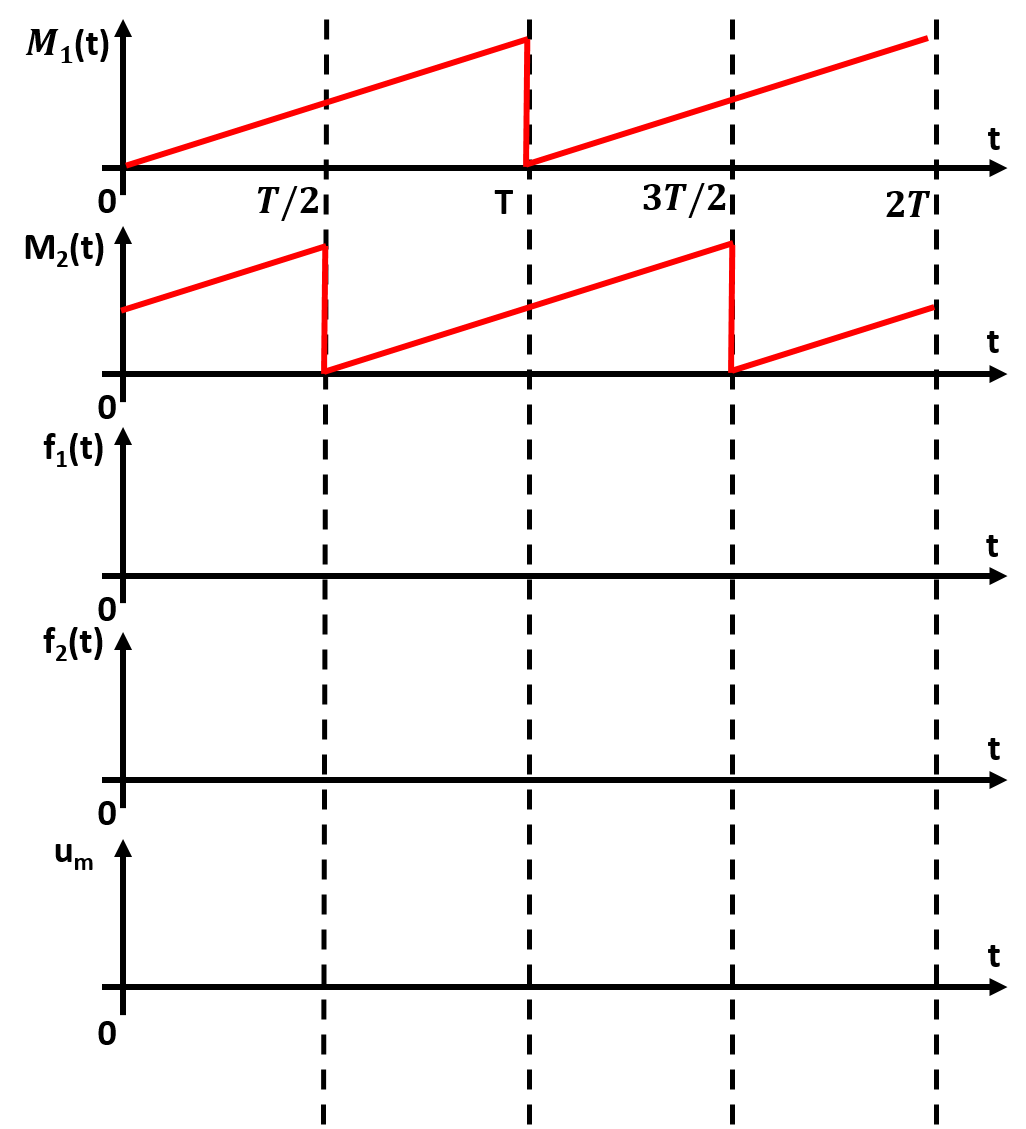
\includegraphics[width=\linewidth]{TD_H4Q/fig/answer.png}
% \caption{Shifted control of a 4 quadrant chopper}
% \end{figure}

%\newpage
%\item \textbf{Independent control}
%
%Here, we propose to change the control of the switches. Transistors $T_{11}$ and $T_{12}$ are still controlled in a complementary manner with the same signal as before. However, transistors $T_{21}$ and $T_{22}$ are now controlled based on the desired output voltage sign: for a positive voltage $U_m$, $T_{22}$ is closed and $T_{21}$ is open, and for a negative voltage $U_m$, $T_{22}$ is open and $T_{21}$ is closed.
%
%\begin{figure}[H]
%\centering
%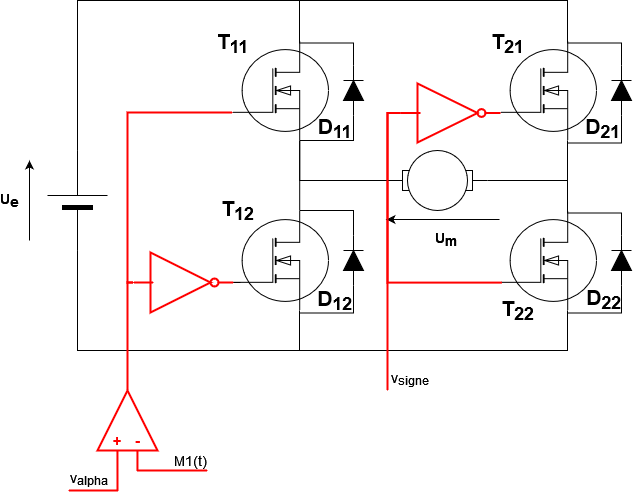
\includegraphics[width=0.6\linewidth]{TD_H4Q/fig/H4Q_indep.png}
%\caption{Independant control 4 quadrant chopper}
%\end{figure}
%
%\begin{enumerate}
%\item Represent the shape of $u_m(t)$ for $\alpha=0.25$ and $v_{signe}=1$
%
%\item Deduce the relationship between the average value of $u_m(t)$ and $\alpha$ when $v_{signe}=1$
%
%\item Represent the shape of $u_m(t)$ for $\alpha=0.25$ and $v_{signe}=0$
%
%\item Deduce the relationship between the average value of $u_m(t)$ and $\alpha$ when $v_{signe}=0$
%
%\item Conclude on the advantages and disadvantages of the different controls
%\end{enumerate}
%
%\begin{figure}[H]
%\centering
%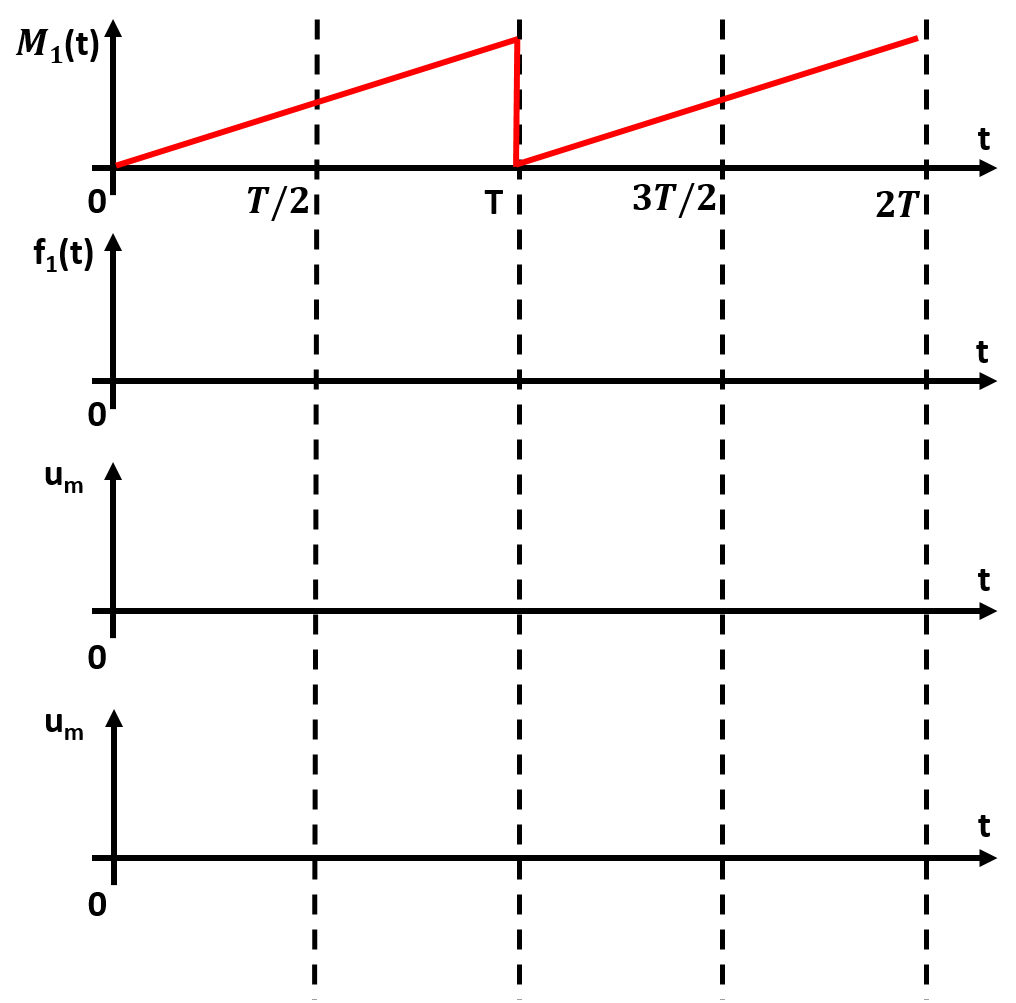
\includegraphics[width=\linewidth]{TD_H4Q/fig/answer2.png}
%%\caption{Shifted control of a 4 quadrant chopper}
%\end{figure}


\end{enumerate}
